% %!TEX root = main.tex
\subsection{Machine to Machine Communication}


\begin{frame}
\frametitle{Publish/Subscribe Protocols}
Pros:

\begin{itemize}
\item Asynchronous communication
\item Decoupling of the communicating entities
\item Many to many
\item Scalable
\end{itemize}

Cons:
\begin{itemize}
\item Semantic coupling (message type needs to be statically defined)
\item Loose message delivery guarantees
\end{itemize}

\end{frame}


\begin{frame}
\frametitle{MQTT}

All of the above plus
\begin{itemize}
\item Lightweight
\item Small code footprint
\item Small header overhead
\item QoS Levels
\end{itemize}

\begin{figure}[!htb]
\centering
\resizebox{0.85\linewidth}{!}{
	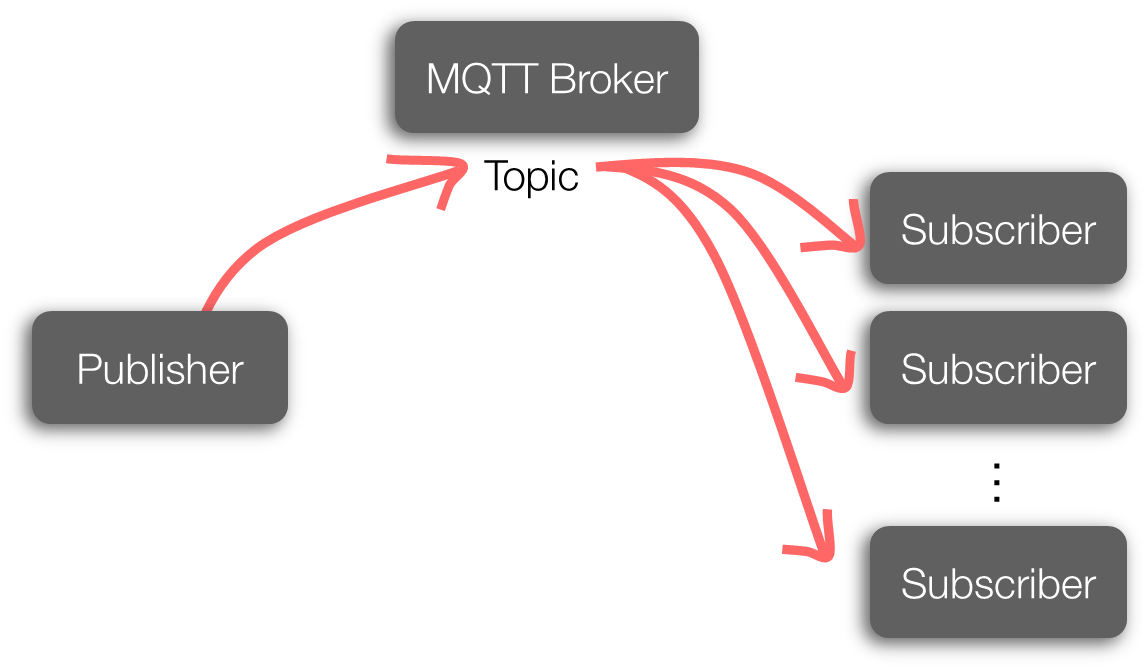
\includegraphics[]{figs/mqtt-block-diagram}
}
\end{figure}

\end{frame}
